\documentclass[tikz]{standalone}
\usepackage{calc}
\usepackage{tikz}
\usetikzlibrary{matrix,fit,backgrounds,calc,decorations.markings,arrows.meta,shapes.geometric,tikzmark,math}
\usepackage{amsmath}
\usepackage{braket}

\begin{document}
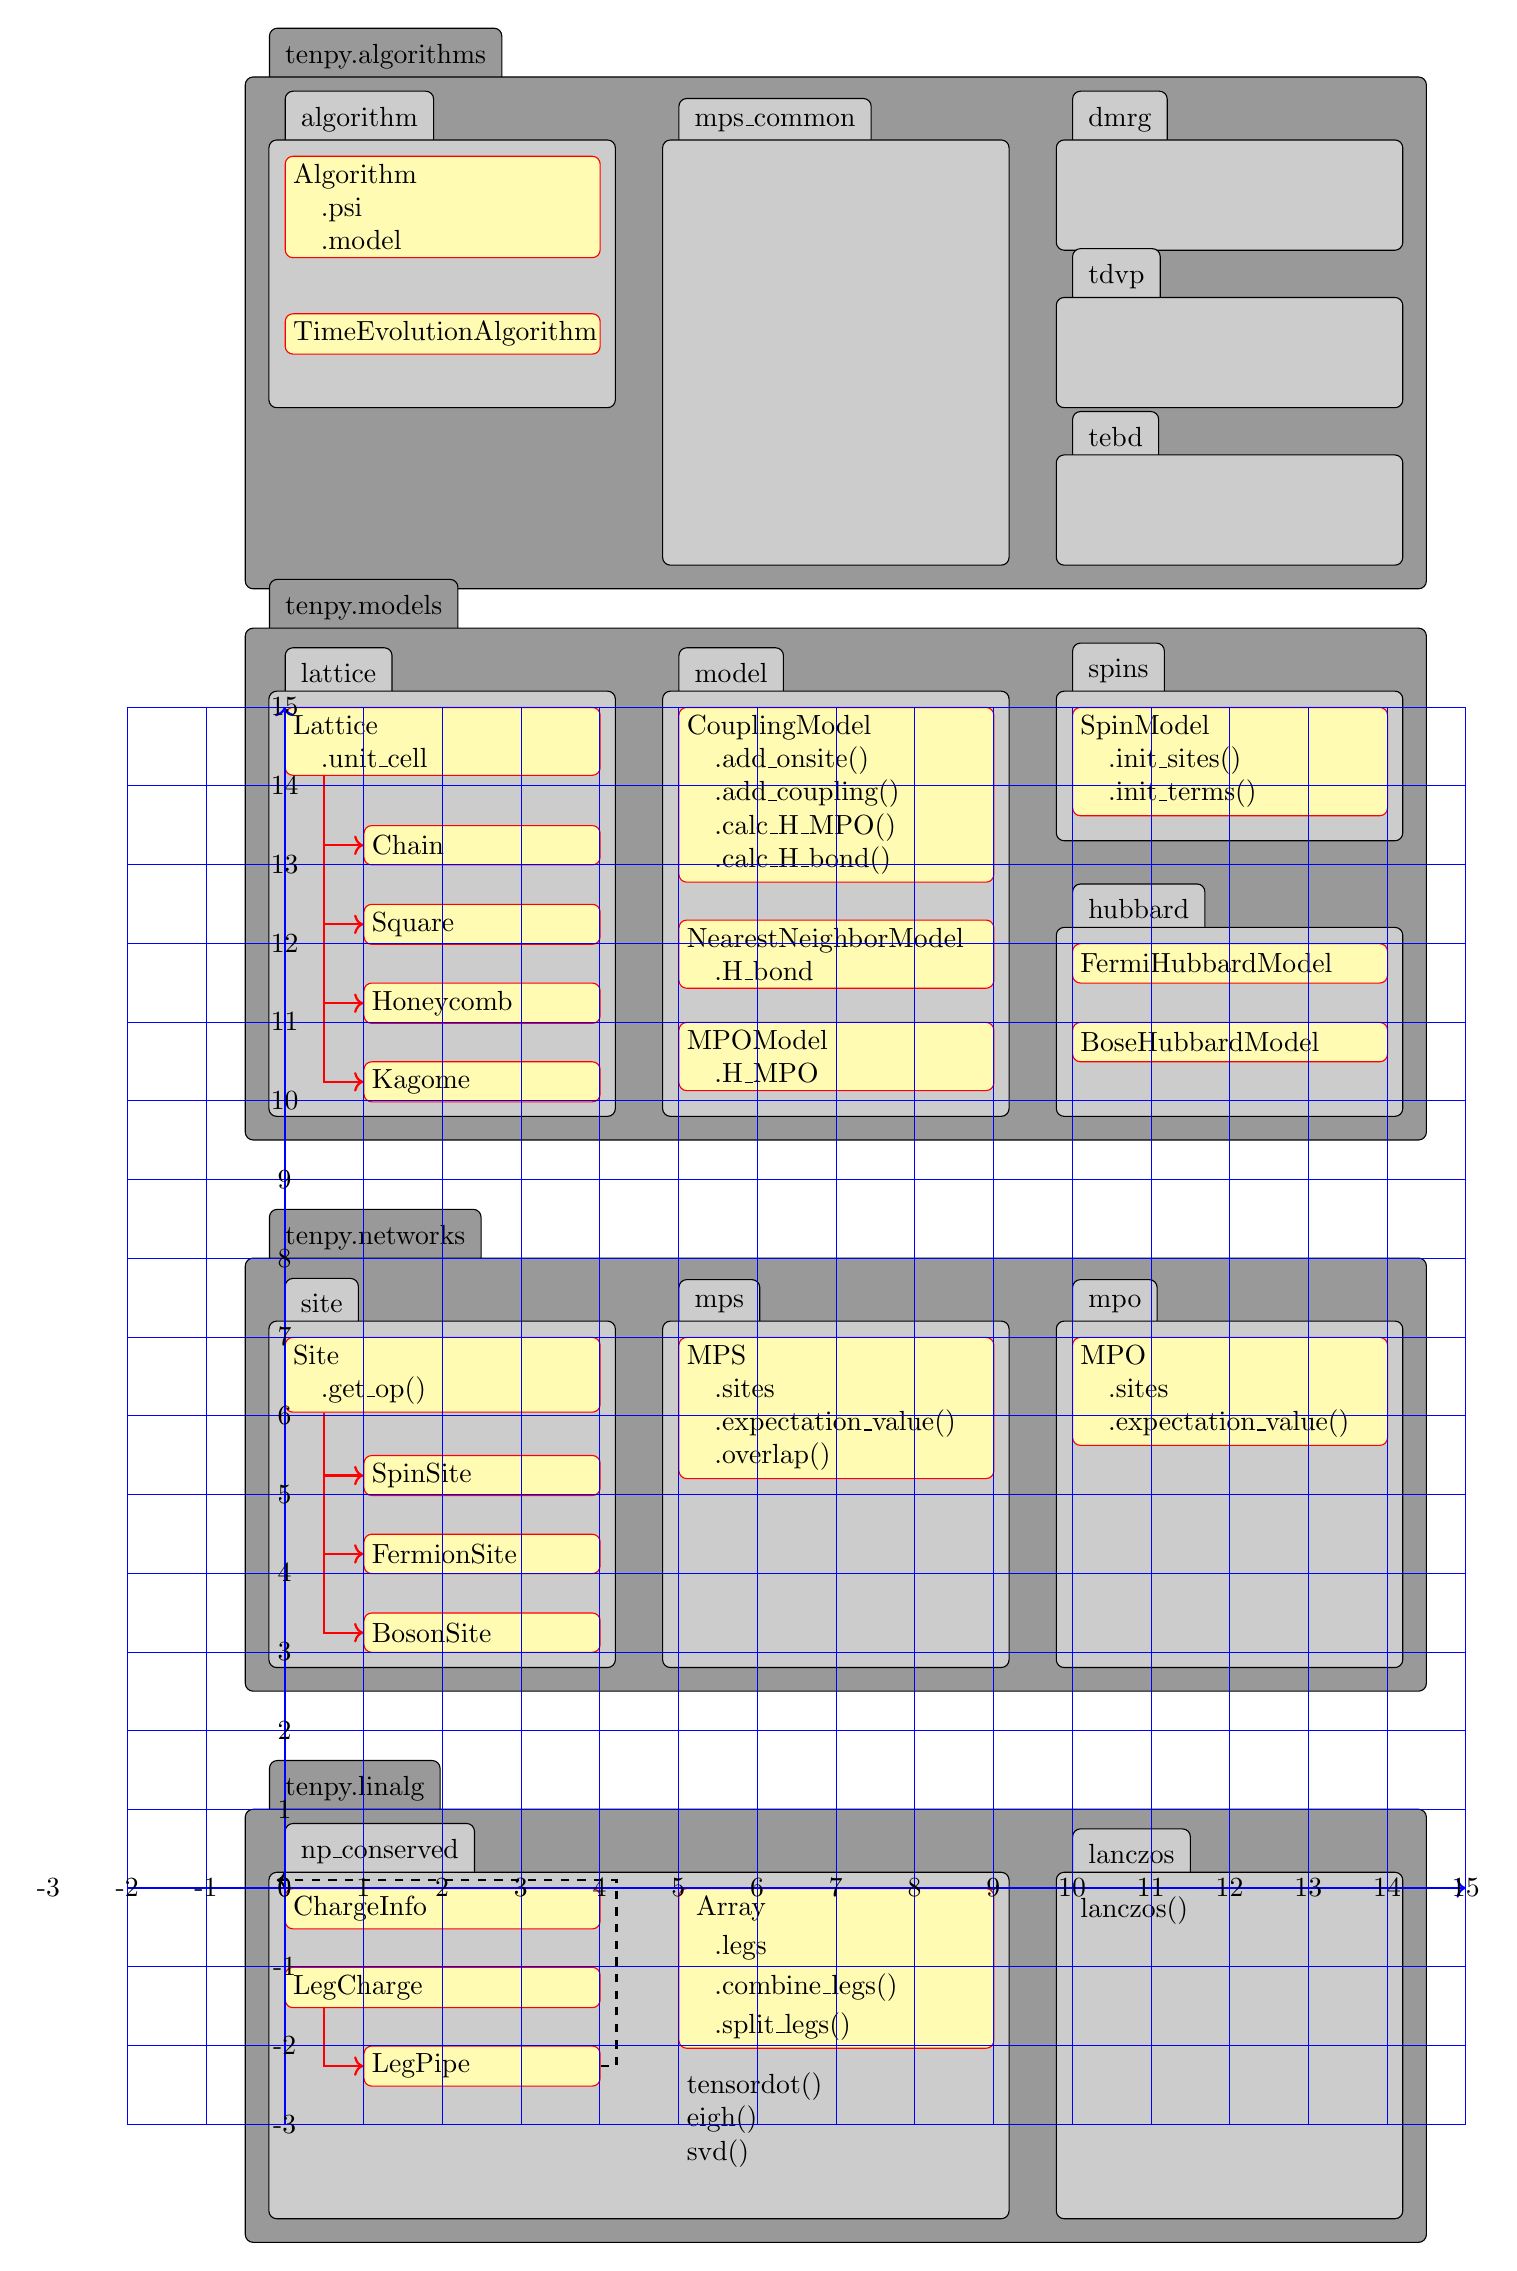
\begin{tikzpicture}[
		remember picture,
		modulecontent/.style={rounded corners=1mm,inner sep=1mm,node font=\texttt,
			minimum height=0.5cm,text width=3.8cm,anchor=north west},
		class/.style={modulecontent,draw=red,fill=yellow!30},
		subclass/.style={class=#1,text width=2.8cm},
		uses/.style={thick,dashed},
		inherit/.style={thick,color=red},
		%
		package/.style={draw,fill=black!40,rounded corners=1mm,inner sep=2mm},
		subpackage/.style={draw,fill=black!20,rounded corners=1mm,inner sep=2mm},
		pics/package/.style n args={2}{code={
			\node[package,anchor=south west] at (-2mm,9mm) {#1};
			\path[package] (-5mm,10mm)  rectangle ($ #2 + (5mm,-5mm)$) ;
		}},
		pics/subpackage/.style n args={2}{code={
			\node[subpackage,anchor=south west] at (0,1mm) {#1};
			\path[subpackage] (-2mm,2mm)  rectangle ($ #2 + (2mm,-2mm)$) ;
		}}%
	]
	\tikzmath{\colw=5; \classw=4; \subind=1; %
		%\cb{n} = class begin{n}; \cs{n} = subclass begin; \ce{n} = class end
		\cb1 = 1*\colw - \colw; \cs1 = \cb1 + \subind; \ce1 = \cb1 + \classw ;
		\cb2 = 2*\colw - \colw; \cs2 = \cb2 + \subind; \ce2 = \cb2 + \classw ;
		\cb3 = 3*\colw - \colw; \cs3 = \cb3 + \subind; \ce3 = \cb3 + \classw ;
	}
	%
	\begin{scope}[yshift=22cm]
		\draw pic at (\cb1, 0) {package={tenpy.algorithms}{(\ce3,-5)}};
		\draw pic at (\cb1, 0) {subpackage={algorithm}{(\ce1,-3)}};
		\draw pic at (\cb2, 0) {subpackage={mps\_common}{(\ce1,-5)}};
		\draw pic at (\cb3, 0) {subpackage={dmrg}{(\ce1,-1)}};
		\draw pic at (\cb3, -2) {subpackage={tdvp}{(\ce1,-1)}};
		\draw pic at (\cb3, -4) {subpackage={tebd}{(\ce1,-1)}};
		% algorithms
		\node[class]   (Algorithm)   at (\cb1, 0  ) {Algorithm \\ \quad  .psi \\ \quad .model };
		\node[class](TimeEvolutionAlgorithm)     at (\cb1,-2.0) {TimeEvolutionAlgorithm};
		% \node[subclass](Square)    at (\cs1,-2.5) {Square};
		% \node[subclass](Honeycomb) at (\cs1,-3.5) {Honeycomb};
		% \node[subclass](Kagome)    at (\cs1,-4.5) {Kagome};
		% % models
		% \node[class]   (CouplingModel) at (\cb2 , 0) {CouplingModel \\
		%     \quad .add\_onsite() \\
		%     \quad .add\_coupling() \\
		%     \quad .calc\_H\_MPO() \\
		%     \quad .calc\_H\_bond() };
		% \node[class]   (NearestNeighborModel) at (\cb2 , -2.7)    {NearestNeighborModel \\
		%     \quad .H\_bond };
		% \node[class]   (MPOModel) at (\cb2 , -4)    {MPOModel \\
		%     \quad .H\_MPO };
		% % spins
		% \node[class]   (SpinModel)          at (\cb3 , 0) {SpinModel \\ \quad .init\_sites() \\ \quad .init\_terms()};
		% \node[class]   (FermiHubbardModel)  at (\cb3 ,-3) {FermiHubbardModel};
		% \node[class]   (BoseHubbardModel)   at (\cb3 ,-4) {BoseHubbardModel};
		% \foreach \subcls in {Chain,Square,Honeycomb,Kagome}
		%     \draw[inherit,->] ($ (Lattice.south west) + (0.5,0) $) |- (\subcls.west) ;
	\end{scope}
	%
	\begin{scope}[yshift=15cm]
		\draw pic at (\cb1, 0) {package={tenpy.models}{(\ce3,-5)}};
		\draw pic at (\cb1, 0) {subpackage={lattice}{(\ce1,-5)}};
		\draw pic at (\cb2, 0) {subpackage={model}{(\ce1,-5)}};
		\draw pic at (\cb3, 0) {subpackage={spins}{(\ce1,-1.5)}};
		\draw pic at (\cb3, -3) {subpackage={hubbard}{(\ce1,-2)}};
		% lattice
		\node[class]   (Lattice)   at (\cb1, 0  ) {Lattice \\ \quad  .unit\_cell };
		\node[subclass](Chain)     at (\cs1,-1.5) {Chain};
		\node[subclass](Square)    at (\cs1,-2.5) {Square};
		\node[subclass](Honeycomb) at (\cs1,-3.5) {Honeycomb};
		\node[subclass](Kagome)    at (\cs1,-4.5) {Kagome};
		% models
		\node[class]   (CouplingModel) at (\cb2 , 0) {CouplingModel \\
			\quad .add\_onsite() \\
			\quad .add\_coupling() \\
			\quad .calc\_H\_MPO() \\
			\quad .calc\_H\_bond() };
		\node[class]   (NearestNeighborModel) at (\cb2 , -2.7)    {NearestNeighborModel \\
			\quad .H\_bond };
		\node[class]   (MPOModel) at (\cb2 , -4)    {MPOModel \\
			\quad .H\_MPO };
		% spins
		\node[class]   (SpinModel)          at (\cb3 , 0) {SpinModel \\ \quad .init\_sites() \\ \quad .init\_terms()};
		\node[class]   (FermiHubbardModel)  at (\cb3 ,-3) {FermiHubbardModel};
		\node[class]   (BoseHubbardModel)   at (\cb3 ,-4) {BoseHubbardModel};
		\foreach \subcls in {Chain,Square,Honeycomb,Kagome}
			\draw[inherit,->] ($ (Lattice.south west) + (0.5,0) $) |- (\subcls.west) ;
	\end{scope}
	%
	\begin{scope}[yshift=7cm]
		\draw pic at (\cb1, 0) {package={tenpy.networks}{(\ce3,-4)}};
		\draw pic at (\cb1, 0) {subpackage={site}{(\ce1,-4)}};
		\draw pic at (\cb2, 0) {subpackage={mps}{(\ce1,-4)}};
		\draw pic at (\cb3, 0) {subpackage={mpo}{(\ce1,-4)}};
		\node[class]   (Site)         at (\cb1 , 0)    {Site \\ \quad  .get\_op() };
		\node[subclass](SpinSite)     at (\cs1, -1.5)   {SpinSite};
		\node[subclass](FermionSite)  at (\cs1, -2.5) {FermionSite};
		\node[subclass](BosonSite)    at (\cs1, -3.5) {BosonSite};
		\node[class]   (MPS)         at (\cb2 , 0)    {MPS \\
			\quad .sites \\
			\quad .expectation\_value() \\
			\quad .overlap() };
		\node[class]   (MPO)         at (\cb3 , 0)    {MPO \\
			\quad .sites \\
			\quad .expectation\_value()};
		%
		\foreach \subcls in {SpinSite,FermionSite,BosonSite}
			\draw[inherit,->] ($ (Site.south west) + (0.5,0) $) |- (\subcls.west) ;
	\end{scope}
	%
	\begin{scope}[yshift=0cm]
		\draw pic at (\cb1, 0) {package={tenpy.linalg}{(\ce3,-4)}};
		\draw pic at (\cb1, 0) {subpackage={np\_conserved}{(\ce2,-4)}};
		\draw pic at (\cb3, 0) {subpackage={lanczos}{(\classw,-4)}};
		\node[class]   (ChargeInfo) at (\cb1, 0) {ChargeInfo};
		\node[class]   (LegCharge)  at (\cb1, -1) {LegCharge};
		\node[subclass](LegPipe)    at (\cs1, -2) {LegPipe};
		%
		\node[class]   (Array)      at (\cb2, 0) {
			\setlength{\baselineskip}{0.5cm}
			Array \\
			\quad \tikzmark{legsin}.legs \\
			\quad .combine\_legs() \\
			\quad .split\_legs() \\
		};
		\node[modulecontent] (npc_fct) at ($ (Array.south west) + (0,-0.2) $) {tensordot() \\ eigh() \\ svd()};
		%
		\node[modulecontent] (Lanczos) at (\cb3, 0) {lanczos()};
		%
		\draw[inherit,->] ($ (LegCharge.south west) + (0.5,0) $) |- (LegPipe.west) ;
		\draw[uses,->] (LegPipe.east) -- +(0.2,0) |- ($ (pic cs:legsin) + (-0.1,0.1) $);
		\draw[uses] (LegPipe.east) -- +(0.2,0) |- ($ (pic cs:legsin) + (-0.1,0.1) $);
	\end{scope}

	% \draw[fill=black] (0,0) rectangle (5,2.5);
	% \node[below,color=white] at (2,2.5) {Hilbert space $\mathcal{H}$};
	% \filldraw[fill=orange!50!white, draw=orange!50!black] (0,0) -- (0.5,0)
	%     arc [start angle=0,end angle=90,radius=0.5] -- cycle;
	% \node[right,color=orange!50!white] (al) at (1,0.4) {area law states} ;
	% \draw[->,color=orange!50!black] (al) -- (0.5,0.2);
	% \fill[color=red] (psi) circle [radius=0.05] ;
	% \node[right,color=red] (psi_lbl) at (0.0,1) {$\ket{\psi_0}$};
	% \draw[->,color=red] (psi_lbl) -- ($(psi_lbl)!0.9!(psi)$) ;
	\draw[very thin, color=blue] (-2.0,-3.0) grid (15.0,15.0);
	\draw[thick,color=blue,->] (-2.,0) -- (15., 0.) ;
	\draw[thick,color=blue,->] (0., -3.) -- (0., 15) ;
	\foreach \i in {-3,...,15}
	{
		\node at (0,\i) {\i{}};
		\node at (\i,0) {\i{}};
	}
\end{tikzpicture}
\end{document}
